\chapter{Background} \label{ch:background}
This chapter includes a background on customer segmentation and clustering algorithms, followed by a background on the use of data analysis, data exploration. The chapter ends with a section on related applications to the software to be created in this project.\par

\section{Customer segmentation}

Customer segmentation or market segmentation tool is widely used in the marketing field. The whole market is divided such that the each segment has similar ``needs, wants or demand''. The organization uses it to target a segment to tailor services to their needs.\par

The four basic market segmentation-strategies: behavioral, based on a person\textsc{\char13}s behavior and decision-making process, demographic, based on the background of an individual such as age, gender, nationality, psychographic, similar to behavioral but is more about the lifestyle and interests, and geographical, based on a person\textsc{\char13}s location \cite{marketing912017}. Local governments usually uses demographic segmentation more than the other types \cite{davey2009}. There are other more complex segmentation approaches involving the customer\textsc{\char13}s interaction with a service or access to a service. However, they are not as prevalent in the public sector \cite{davey2009}. Clustering algorithms could also be used to identify the segments \cite{lgaguide}. \par

The resources of an organization are limited and it usually cannot cater for the whole population. The private and public sector have to approach customer segmentation differently as the private sector aims to maximize business and targets the specific segments of the population. This is contrary to the public sector which has the mandate to cater to the whole population. They focus more on offering appropriate services to segments of the population. Policies usually targets segments of the population, where the minorities may not experience the benefits and only the majority of the population do.\par

Customer segmentation is a concept promoted by the national government and the Local Government Association (LGA) has created a guidance document for any council that wishes to implement such a tool \cite{lgaguide}. They give guidance on which data sets to use, segmentation of the population with k-means clustering and ways to visualize the data. Explicit data about its customers is combined with implicit data ``knowledge of staff on customers using a service'' \cite{smartcities}. This would give a more complete view on not only the customers\textsc{\char13} profile but also their behaviors in interacting with the service.\par

\section{Clustering}

Clustering is a task which aims to group data points in an unlabeled data set where each point within a group, called a cluster, is more similar to another point in another cluster. It can be implemented as different algorithms using varying methods of determining similarity. The number of clusters is determined by the user depending on their expectations from the data. It has numerous applications in different fields such as data science, biology, medicine and business to name a few. It is also a technique used in customer segmentation where a clustering algorithm can label the segments within a collection of market data \cite{lgaguide}. \par


The optimal number of clusters is subjective however, there are ways to determine the best number of clusters to use. One method, the elbow method, requires a graph of the percentage of variance and the number of clusters \cite{thedatasciencelab2014}. The sum of the intra-cluster distances between points in a cluster. The normalized intra-cluster sum of squares gives the variance quantity. The percentage variance is calculated as the ratio of the between-group variance to the total variance. As the number of clusters increases the percentage of variance increases significantly until a certain point, which creates a bend. In this method, the clearest bend in the graph determines most suitable number of clusters, however finding the bend may be an ambiguous task as it depends on the clarity of the bend.\par

There are different measures to determine if data points should form a cluster which include the structure of a cluster through closeness but also the concept of the cluster. Distance, metrics such as Euclidian, cosine, Jaccard, Hamming distance, Manhattan \cite{oneilschutt2014}. An implementation of this is the k-means algorithm which uses Euclidian distance to calculate similarity. However, it is not as preferable for clustering categorical data. Euclidian distance calculates a mean which could relate two discrete values or categories together. Huang\textsc{\char13}s k-modes \cite{Huang1998} is an algorithm to avoid this issue. It instead matches categorical data of different data points through the calculation of the mode, respecting the categories as discrete values, rather than the contrary in Euclidean distance. \par

There are other ways of clustering through structure which involve density includes a point such that it does not exceed density of points within the radius of a cluster \cite{tutorialspoint}. Conceptual clustering uses a descriptive language to define the concepts of the cluster through instead of similarity measures \cite{clusteringintroduction}. The descriptive language defines the model in which to compare the similarity of data points.\par

\section{Data science}
Data science is a multi-disciplinary field which intends to ``analyze and understand actual phenomena'' \cite{Hayashi1998} but it also deals with the communication of its results \cite{oneilschutt2014}. It is multi-disciplinary because it not only involves statistical data analysis, but also domain expertise, data visualization, machine learning which are skills needed in this field.\par

In the field of data science, data exploration is one of the steps in the data science process. After data is collected from the real world, processed and cleaned, which converts raw data into a usable format. Depending on the process used, the next step is either data exploration \cite{oneilschutt2014} or stating the question followed by data exploration \cite{peng2016}.\par

Nevertheless, though the order may be different, both process agree that data science involves exploring the data, building models, interpreting and then communicating the results. These steps demonstrate the need for different disciplines in this field as statistics and domain expertise is required in building models and data visualization is required for communicating the results.\par

\subsection{Data exploration}
Data exploration aids the user in understanding the structure of the data set, discovering if there are missing values, examining the distributions of individual variables, to name a few. O'Neil and Schutt \cite{oneilschutt2014} explains that data exploration is not only about confirming expectations or hypotheses but also to discover new information which one did not expect. Tools include plots, graphs and summary statistics. Data visualization through plots such as boxplots and graphs allows one to absorb information and identify patterns more easily. Summary statistics involve simple statistical data such as a variable\textsc{\char13}s mean, median, mode and range.

\section{Related works}

This subsection describes some works related to the software created in this project, which includes academic research of prototypes for data exploration, customer segmentation tools and government websites which visualize data. There are other related tools, however, reviewing all of them is beyond the scope of this report.
\par

\subsection{Data exploration tools}

Gogolou et al. \cite{gogoloudata2016} created prototype, Data Curation and Validation (DCV) which supports user-data interaction especially in data cleaning and exploration. DCV, originally a data cleaning tool, has lead them to believe that any interaction with the data is data exploration. Therefore, the tool has been expanded to include data exploration features. There are three components, the presentation, visualization and profiling. The presentation component allows the user to select the type of visualization they wish to see on a variable. The profiling component predicts if there is erroneous data such as outliers and recommends actions to the user according to previous data analysis. The activity component deals with data exploration tasks such as data search and analysis.\par

Similarly, Graves and Hendler \cite{gravesvisualization2013} created a prototype which allows users with no technical expertise, but more specifically targeted to visualize open government data (OGD). Ordinary citizens, journalists, those with no experience in consuming OGD are at a disadvantage. Visualizations enables an ordinary person to consume large amounts of data. Therefore, creating visualizations of OGD will enable them to consume this data. They identified groups of software which deal with this problem namely, office suits, business intelligence software, specialized analysis tools and visualization APIs which are not suitable for the consumption of OGD by the layman. They discuss what is needed in such a software: simplification of the visualization process, providing meta-data about the current data set such as location, time of creation, understandable conventions on description of data (i.e. turn FY1998 into its worded description), including the contact information of the provider, sharing visualizations on social networks.\par

The neighborhood statistics website \cite{neighbourhoodstatistics} of the UK government gives a summary and visualizes some census data. The website enables the user to view census data on a geographical area. The user can view a data set as a table or on a map (see figure \ref{fig:neighborhood}). The table shows aggregation of the data set where each row represents a variable. The map visualizes the values of the selected variable through different shades of color according to the legend. A time series graph also allows the user to view differences of the aggregate value over the years. The tool however limits the user to viewing only one variable at a time.\par

\begin{figure}[h]
\centering
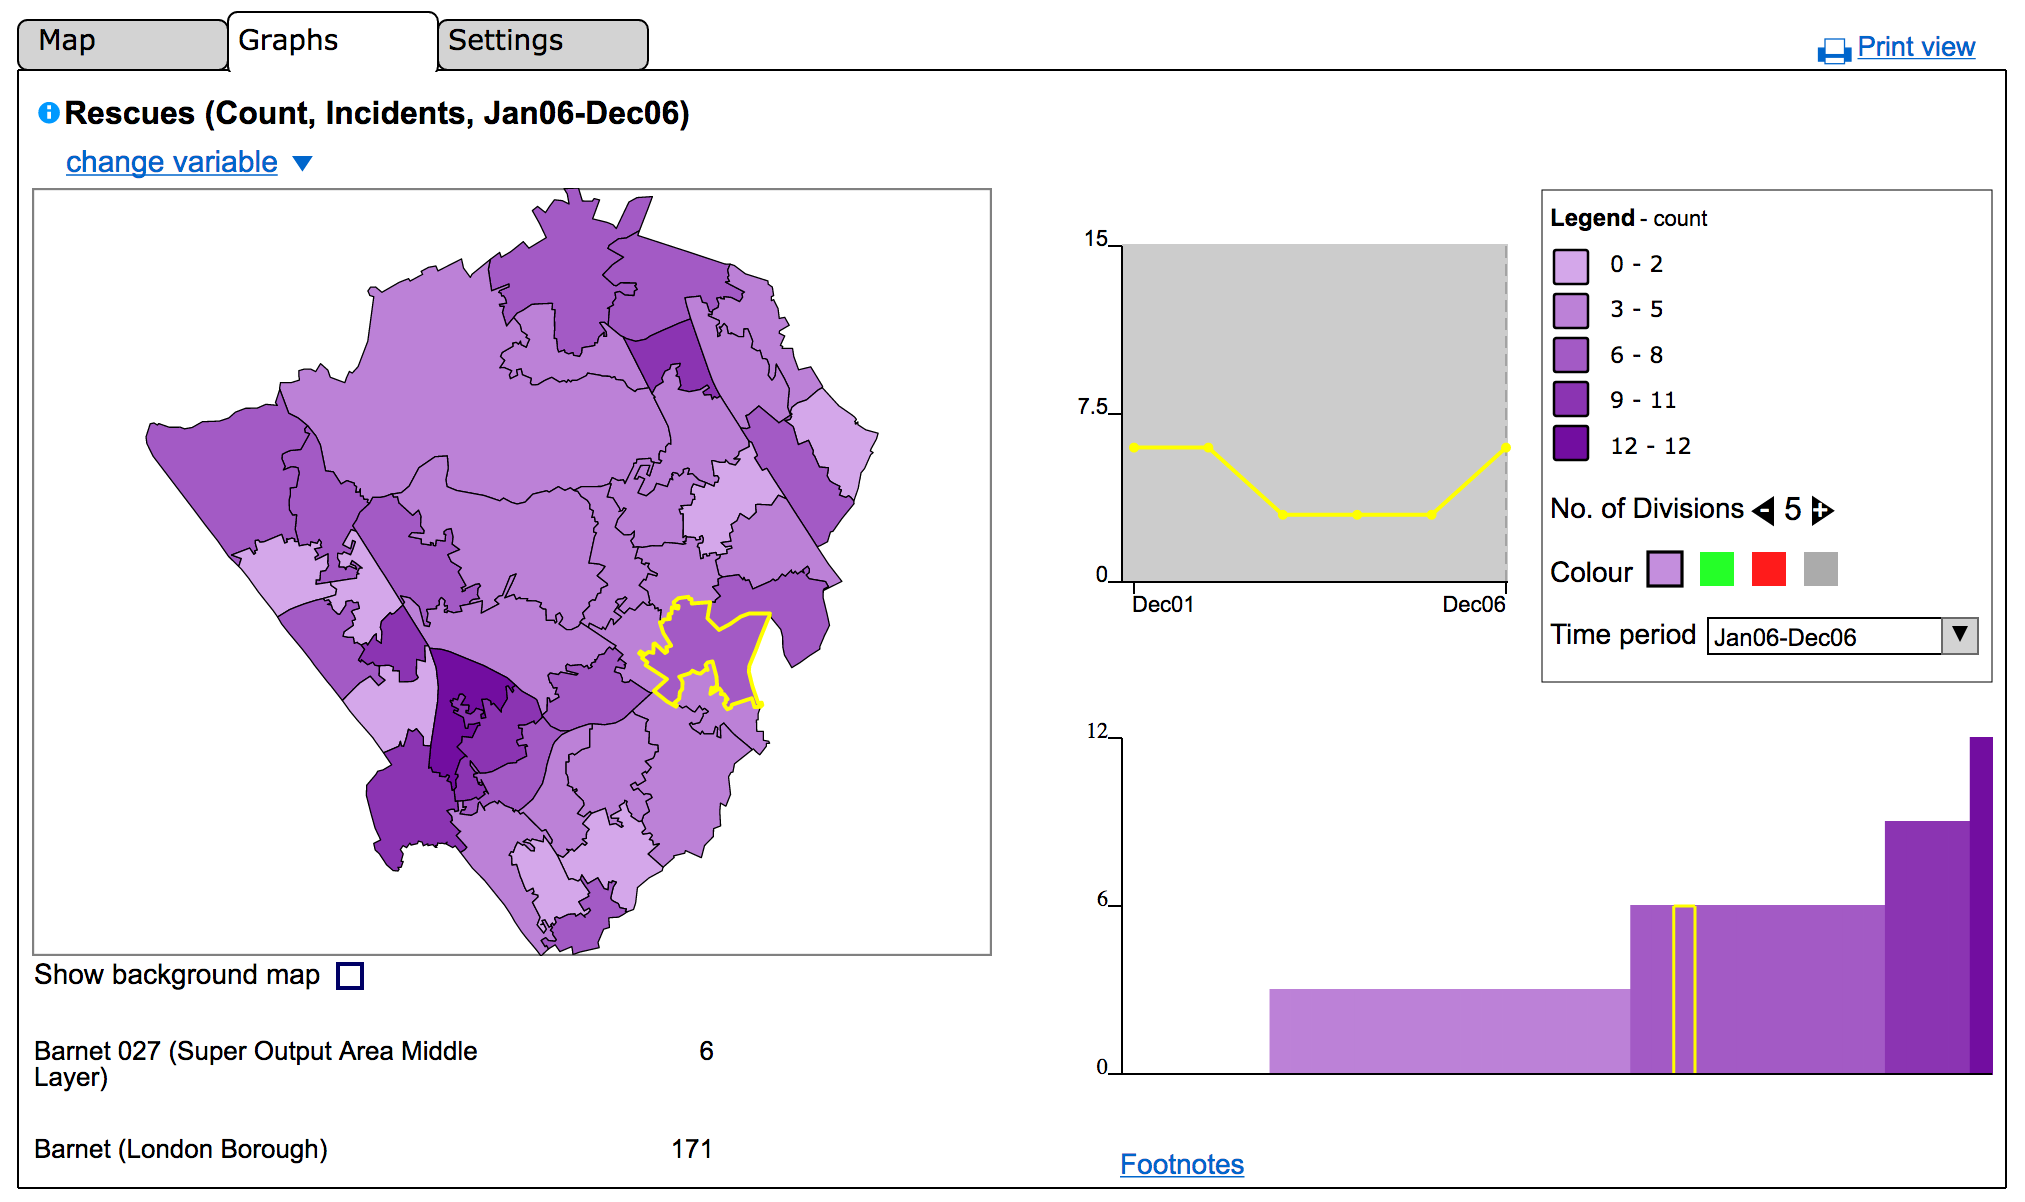
\includegraphics[scale=0.3]{neighborhood}
\caption{Screenshot of a page in neighbourhood.statistics.co.uk}
\label{fig:neighborhood}
\end{figure}

\subsection{Customer segmentation tools}

There are tools which presents pre-made customer segmentation analysis of the UK population like Mosaic Public Sector by Experian \cite{experian}, Acorn by CACI \cite{acornuserguide} and Kent \& Medway\textsc{\char13}s interactive guide \cite{kentmidway}. \par

Mosaic Public Sector uses government data and visualizes this data through an interactive tool intended for public sector use. The tool has pre-made customer groups using their data and the visualizations include maps, photos and graphs. It utilizes data from different sources, from census to social media data to create the segments. \par

On the other hand, Acorn uses government but also commercially available data. Like Mosaic, it has created pre-made customer segments. However, there is a feature that enables the user to find out more about their customer through just their post code. This approach separates itself from matching demographic classifications to locations to matching locations to demographic types. \par

Kent \& Medway tool which visualizes the segments its population by social class determined by the council\textsc{\char13}s own customer segmentation analysis. It has a feature which compares a data variable between all groups of the population (see figure \ref{fig:kent}).\par

There have been similarities between implemented tools and recommendations to differentiate and describe each group. Kent \& Medway suggested to include maps showing the concentration of that group in each ward and in addition to a textual description, they include pictures to describe each group. It also includes graphs to visualize data but also word maps of key characteristics. The LGA guide \cite{lgaguide} has suggested that the use of spider diagrams which detail the variables compared to the town and district average. Similarly Kent \& Medway and Acorn, they graph pieces of data with an index of the group compared to the overall population. This visualizes both the average value and the groups relation to that average displays whether they are higher or lower than that average however each graph is created for each variable.


\begin{figure}[h]
\centering
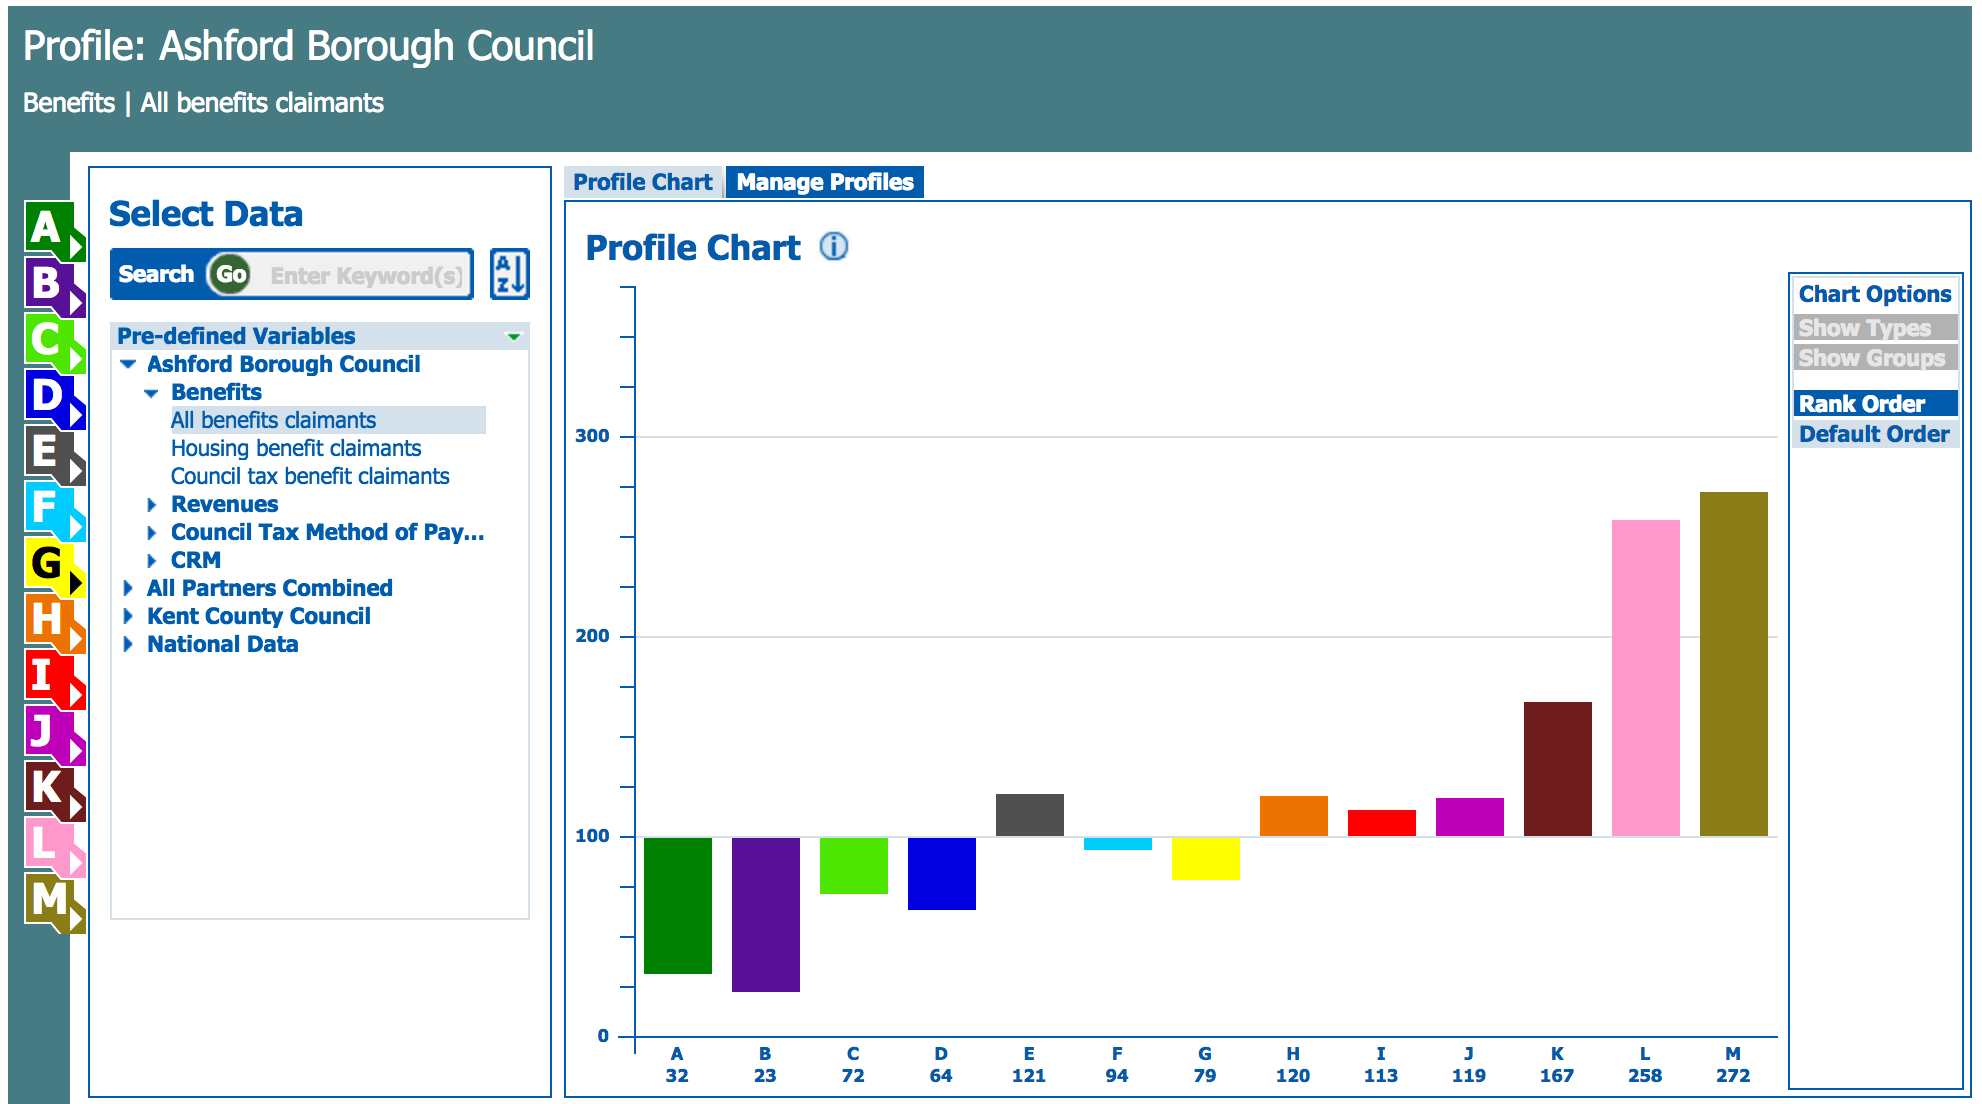
\includegraphics[scale=0.3]{kent}
\caption{Screenshot of a page in Kent \& Medway interactive site}
\label{fig:kent}
\end{figure}